\documentclass{beamer}
\usepackage[utf8]{inputenc}
\usetheme{Singapore}
\title[Git]{Introduction to Git}
\author{Florian Schulz}
\begin{document}

\begin{frame}
\titlepage
\end{frame}

%\begin{frame}{Geschichte}
%\end{frame}

\begin{frame}{Git vs. SVN (SVN)}
\begin{figure} 
\centering
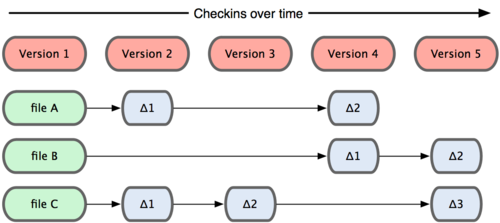
\includegraphics{images/18333fig0104-tn.png}
\end{figure}
\end{frame}

\begin{frame}{Git vs. SVN (Git)}
\begin{figure} 
\centering
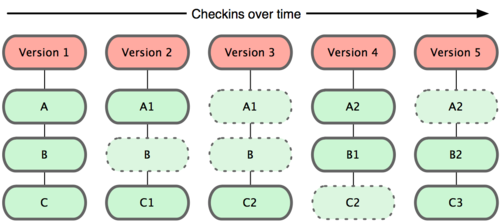
\includegraphics{images/18333fig0105-tn.png}
\end{figure}
\end{frame}

\begin{frame}{Git vs. SVN (Git)}
\end{frame}

\begin{frame}{Standardworkflow (wie SVN)}
git clone git://github.com/schacon/grit.git $\langle$directory$\rangle$
\begin{figure} 
\centering
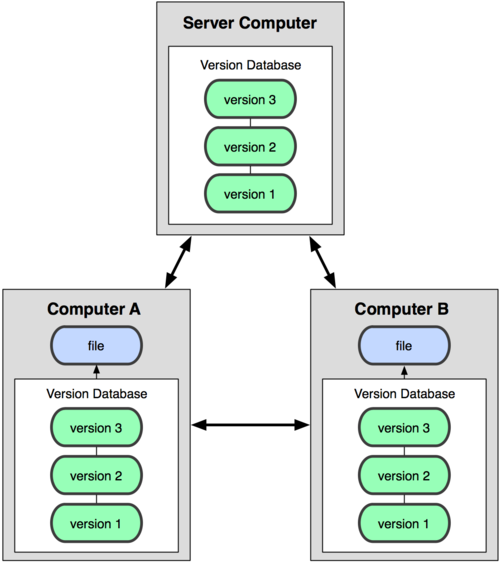
\includegraphics[scale=0.5]{images/18333fig0103-tn.png}
\end{figure}
\end{frame}

\begin{frame}{Standardworkflow (wie SVN)}
git status
\begin{figure} 
\centering
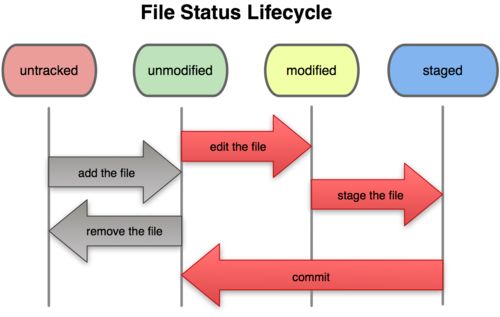
\includegraphics[scale=0.5]{images/18333fig0201-tn.png}
\end{figure}
\end{frame}


\begin{frame}{Branching/Merging/Rebasing}
\end{frame}



\end{document}